\documentclass[11pt,a4paper]{article}

\usepackage[utf8]{inputenc}
\usepackage[T1]{fontenc}
\usepackage[brazil]{babel}
\usepackage{geometry}
\usepackage{booktabs}
\usepackage{xcolor}
\usepackage{graphicx}
\usepackage{float}
\usepackage{caption}
\usepackage{enumitem}
\usepackage{hyperref}

\geometry{top=2cm,bottom=2cm,left=2.2cm,right=2.2cm}
\setlist{itemsep=2pt, topsep=2pt}
\hypersetup{colorlinks=true,linkcolor=blue!70!black,citecolor=blue!70!black,urlcolor=blue!70!black}
\graphicspath{{../results/}}

\title{\vspace{-1.2cm}Classificação de Emoções em Tweets com Encoders Transformer Congelados\\
\large PCS3838 Inteligência Artificial, Trabalho Prático}
\author{
André Moreno (13682785) \and Giovani Sebastianutti (13680171) \and Matheus Guidoni (12683120)
}
\date{Escola Politécnica da USP, novembro de 2026}

\begin{document}
\maketitle

\section{Conjunto de dados}

Usamos o \textit{Emotion Dataset}, distribuído no Kaggle por Parul Pandey\footnote{\url{https://www.kaggle.com/datasets/parulpandey/emotion-dataset}} a partir da versão publicada pela DAIR.AI no Hugging Face Hub (\texttt{dair-ai/emotion}). Os dados vêm do trabalho de Saravia, Liu, Huang, Wu e Chen, \textit{CARER: Contextualized Affect Representations for Emotion Recognition}, apresentado no EMNLP 2018.

A finalidade original foi estudar o reconhecimento de emoções em textos curtos e informais de redes sociais. Os autores propuseram representações baseadas em padrões de grafos para capturar expressões emocionais além do vocabulário isolado, e precisaram para isso de um corpus grande rotulado.

A construção se deu por supervisão distante. Tweets em inglês foram coletados pela API do Twitter e o rótulo de emoção foi atribuído a partir de hashtags associadas a cada emoção. As hashtags usadas como rótulo foram depois removidas do texto, para que o classificador não aprendesse o rótulo diretamente. Os textos foram normalizados: estão todos em minúsculas, sem pontuação, sem menções e sem URLs. Uma característica marcante é que 98,8\% dos textos contêm alguma forma de ``feel'' (``i feel'', ``im feeling''), o que reflete o padrão de coleta. Os rótulos são, portanto, ruidosos: dependem da hashtag que o próprio autor do tweet escolheu, e não de anotação humana independente.

A versão usada tem 20.000 textos divididos em treino (16.000), validação (2.000) e teste (2.000), com seis classes. Como o enunciado pede validação cruzada, juntamos as três partes. A Tabela~\ref{tab:classes} mostra a distribuição. O desbalanceamento é forte: \textit{joy} e \textit{sadness} somam 62\% e \textit{surprise} tem 3,6\%. Os textos têm em média 19 palavras (mediana 17, máximo 66). Há 52 textos repetidos, número pequeno demais para afetar as métricas.

\begin{table}[H]
\centering
\caption{Distribuição das classes (20.000 textos).}
\label{tab:classes}
\begin{tabular}{lrrrrrr}
\toprule
& sadness & joy & love & anger & fear & surprise \\
\midrule
Rótulo & 0 & 1 & 2 & 3 & 4 & 5 \\
Textos & 5.797 & 6.761 & 1.641 & 2.709 & 2.373 & 719 \\
\% & 29,0 & 33,8 & 8,2 & 13,5 & 11,9 & 3,6 \\
\bottomrule
\end{tabular}
\end{table}

\section{Encoders}

Escolhemos três encoders de propósito geral para inglês, todos de tamanho \textit{base} (12 camadas, dimensão oculta 768), nenhum ajustado para emoções ou para este dataset.

\begin{itemize}
\item \texttt{bert-base-uncased}: BERT, de Devlin, Chang, Lee e Toutanova (Google, NAACL 2019). Introduziu o pré-treino bidirecional com modelagem de linguagem mascarada (MLM) e predição da próxima sentença. Treinado em BookCorpus e Wikipédia em inglês, com vocabulário WordPiece de 30 mil tokens e 110M de parâmetros. A versão \textit{uncased} combina com o texto todo em minúsculas do dataset.
\item \texttt{roberta-base}: RoBERTa, de Liu et al. (Facebook AI, 2019). Mantém a arquitetura do BERT e revisa o pré-treino: remove a predição da próxima sentença, usa mascaramento dinâmico, lotes maiores e cerca de 160 GB de texto (dez vezes mais), incluindo notícias e texto da web. Usa BPE em nível de byte com 50 mil tokens (125M de parâmetros).
\item \texttt{microsoft/deberta-v3-base}: DeBERTa-v3, de He, Gao e Chen (Microsoft, ICLR 2023). Herda do DeBERTa a atenção desacoplada, que representa conteúdo e posição relativa em vetores separados. A novidade da v3 é trocar o MLM pela detecção de token substituído do ELECTRA, em que um gerador pequeno troca tokens e o modelo aprende a apontar quais foram trocados, com compartilhamento de embeddings desacoplado por gradiente entre gerador e discriminador. Vocabulário SentencePiece de 128 mil tokens (86M de parâmetros no corpo e 98M na camada de embeddings).
\end{itemize}

\section{Procedimentos e parâmetros}

\paragraph{Vetor por texto.} Os encoders ficaram congelados (modo \texttt{eval} e \texttt{torch.no\_grad}, sem atualização de pesos). Cada texto foi tokenizado com truncamento em 128 tokens (nenhum texto chega perto disso) e passado pelo encoder em lotes de 64 em GPU. O vetor do texto é a média dos estados ocultos da última camada sobre os tokens reais, usando a \texttt{attention\_mask} para ignorar o padding. Preferimos a média ao token \texttt{[CLS]} porque, sem ajuste fino, o \texttt{[CLS]} não é treinado para resumir a frase (no RoBERTa e no DeBERTa-v3 ele não tem nenhum objetivo próprio no pré-treino). Cada encoder gera uma matriz $20.000 \times 768$, salva em disco.

\paragraph{Classificadores.} Ambos usam \texttt{StandardScaler} seguido do classificador, dentro de um \texttt{Pipeline}, de modo que a padronização é ajustada só no treino de cada fold.
\begin{itemize}
\item Regressão logística: multinomial, solver \texttt{lbfgs}, regularização L2 com $C=1$, \texttt{max\_iter=3000} para garantir convergência.
\item MLP: uma camada oculta de 256 neurônios ReLU, otimizador Adam com taxa inicial $10^{-3}$, lotes de 200, regularização L2 \texttt{alpha}$=10^{-3}$, \textit{early stopping} com 10\% do treino do fold separado como validação interna e paciência de 10 épocas, \texttt{max\_iter=300}.
\end{itemize}
A regressão logística funciona como sonda linear: mede quanto da emoção é linearmente separável na representação. O MLP testa se uma fronteira não linear extrai mais informação dos mesmos vetores. Não fizemos busca de hiperparâmetros, para manter as seis configurações sob as mesmas condições, e não usamos pesos por classe porque o \texttt{MLPClassifier} não oferece essa opção. A semente aleatória é 42 em todo o experimento.

\paragraph{Validação cruzada.} \texttt{StratifiedKFold} com 5 folds, embaralhamento e semente fixa. Os índices dos folds foram gerados uma única vez, salvos e reutilizados nas seis configurações, então todas são avaliadas exatamente nas mesmas partições. A estratificação mantém a proporção das classes em cada fold, o que é importante aqui por causa da classe \textit{surprise}, com cerca de 144 exemplos por fold. Uma limitação do método é assumir exemplos independentes e identicamente distribuídos: textos quase duplicados ou de um mesmo autor podem cair em folds diferentes e inflar levemente as métricas. Além disso, 5 folds dão uma estimativa de variância com poucos pontos.

\paragraph{Métricas.} Para cada fold calculamos acurácia e precisão, recall e F1 em média macro (todas as classes com o mesmo peso), e reportamos média e desvio-padrão amostral entre os folds. As matrizes de confusão usam as predições de validação de todos os folds (\textit{out-of-fold}): cada texto aparece uma única vez, predito por um modelo que não o viu no treino.

\section{Resultados}

A Tabela~\ref{tab:consolidada} consolida as seis configurações e a Tabela~\ref{tab:folds} mostra os valores por fold. A Figura~\ref{fig:cm} traz as matrizes de confusão normalizadas por linha. O notebook contém também as matrizes com contagens absolutas.

\begin{table}[H]
\centering
\caption{Tabela consolidada: média $\pm$ desvio-padrão em 5 folds (precisão, recall e F1 em média macro), ordenada por F1.}
\label{tab:consolidada}
\begin{tabular}{lcccc}
\toprule
Configuração & Acurácia & Precisão & Recall & F1 \\
\midrule
RoBERTa + MLP       & 0,654 $\pm$ 0,010 & 0,595 $\pm$ 0,012 & 0,552 $\pm$ 0,018 & 0,569 $\pm$ 0,016 \\
RoBERTa + LogReg    & 0,645 $\pm$ 0,010 & 0,572 $\pm$ 0,009 & 0,554 $\pm$ 0,009 & 0,561 $\pm$ 0,009 \\
BERT + MLP          & 0,645 $\pm$ 0,008 & 0,580 $\pm$ 0,012 & 0,545 $\pm$ 0,013 & 0,558 $\pm$ 0,012 \\
BERT + LogReg       & 0,636 $\pm$ 0,005 & 0,561 $\pm$ 0,012 & 0,538 $\pm$ 0,009 & 0,547 $\pm$ 0,009 \\
DeBERTa-v3 + LogReg & 0,585 $\pm$ 0,004 & 0,491 $\pm$ 0,008 & 0,462 $\pm$ 0,008 & 0,472 $\pm$ 0,008 \\
DeBERTa-v3 + MLP    & 0,566 $\pm$ 0,008 & 0,480 $\pm$ 0,024 & 0,431 $\pm$ 0,013 & 0,443 $\pm$ 0,011 \\
\bottomrule
\end{tabular}
\end{table}

\begin{table}[H]
\centering
\small
\caption{Métricas por fold (A: acurácia, P: precisão, R: recall, F1, em média macro).}
\label{tab:folds}
\setlength{\tabcolsep}{4pt}
\begin{tabular}{l|cccc|cccc|cccc}
\toprule
& \multicolumn{4}{c|}{BERT + LogReg} & \multicolumn{4}{c|}{RoBERTa + LogReg} & \multicolumn{4}{c}{DeBERTa-v3 + LogReg} \\
Fold & A & P & R & F1 & A & P & R & F1 & A & P & R & F1 \\
\midrule
1 & ,637 & ,564 & ,540 & ,549 & ,644 & ,568 & ,546 & ,556 & ,588 & ,496 & ,473 & ,482 \\
2 & ,636 & ,568 & ,544 & ,553 & ,641 & ,572 & ,558 & ,563 & ,578 & ,484 & ,461 & ,470 \\
3 & ,640 & ,570 & ,536 & ,549 & ,660 & ,588 & ,565 & ,575 & ,589 & ,491 & ,455 & ,467 \\
4 & ,627 & ,541 & ,525 & ,531 & ,647 & ,571 & ,555 & ,562 & ,582 & ,481 & ,456 & ,463 \\
5 & ,638 & ,561 & ,547 & ,553 & ,633 & ,562 & ,544 & ,552 & ,586 & ,501 & ,465 & ,477 \\
\midrule
& \multicolumn{4}{c|}{BERT + MLP} & \multicolumn{4}{c|}{RoBERTa + MLP} & \multicolumn{4}{c}{DeBERTa-v3 + MLP} \\
Fold & A & P & R & F1 & A & P & R & F1 & A & P & R & F1 \\
\midrule
1 & ,656 & ,593 & ,567 & ,578 & ,660 & ,604 & ,565 & ,581 & ,565 & ,472 & ,443 & ,452 \\
2 & ,636 & ,567 & ,536 & ,549 & ,650 & ,596 & ,552 & ,569 & ,566 & ,471 & ,435 & ,445 \\
3 & ,644 & ,575 & ,533 & ,549 & ,668 & ,607 & ,569 & ,584 & ,574 & ,484 & ,442 & ,455 \\
4 & ,649 & ,593 & ,542 & ,562 & ,642 & ,580 & ,522 & ,543 & ,555 & ,454 & ,422 & ,432 \\
5 & ,642 & ,573 & ,545 & ,555 & ,651 & ,585 & ,555 & ,565 & ,573 & ,518 & ,414 & ,431 \\
\bottomrule
\end{tabular}
\end{table}

\begin{table}[H]
\centering
\caption{F1 por classe, calculado sobre as predições \textit{out-of-fold}.}
\label{tab:perclass}
\begin{tabular}{lcccccc}
\toprule
Configuração & sadness & joy & love & anger & fear & surprise \\
\midrule
RoBERTa + MLP       & 0,695 & 0,745 & 0,416 & 0,582 & 0,558 & 0,418 \\
RoBERTa + LogReg    & 0,686 & 0,741 & 0,408 & 0,565 & 0,563 & 0,407 \\
BERT + MLP          & 0,693 & 0,740 & 0,418 & 0,555 & 0,545 & 0,403 \\
BERT + LogReg       & 0,679 & 0,739 & 0,398 & 0,543 & 0,531 & 0,393 \\
DeBERTa-v3 + LogReg & 0,630 & 0,714 & 0,278 & 0,454 & 0,463 & 0,293 \\
DeBERTa-v3 + MLP    & 0,608 & 0,708 & 0,238 & 0,408 & 0,436 & 0,268 \\
\bottomrule
\end{tabular}
\end{table}

\begin{figure}[H]
\centering
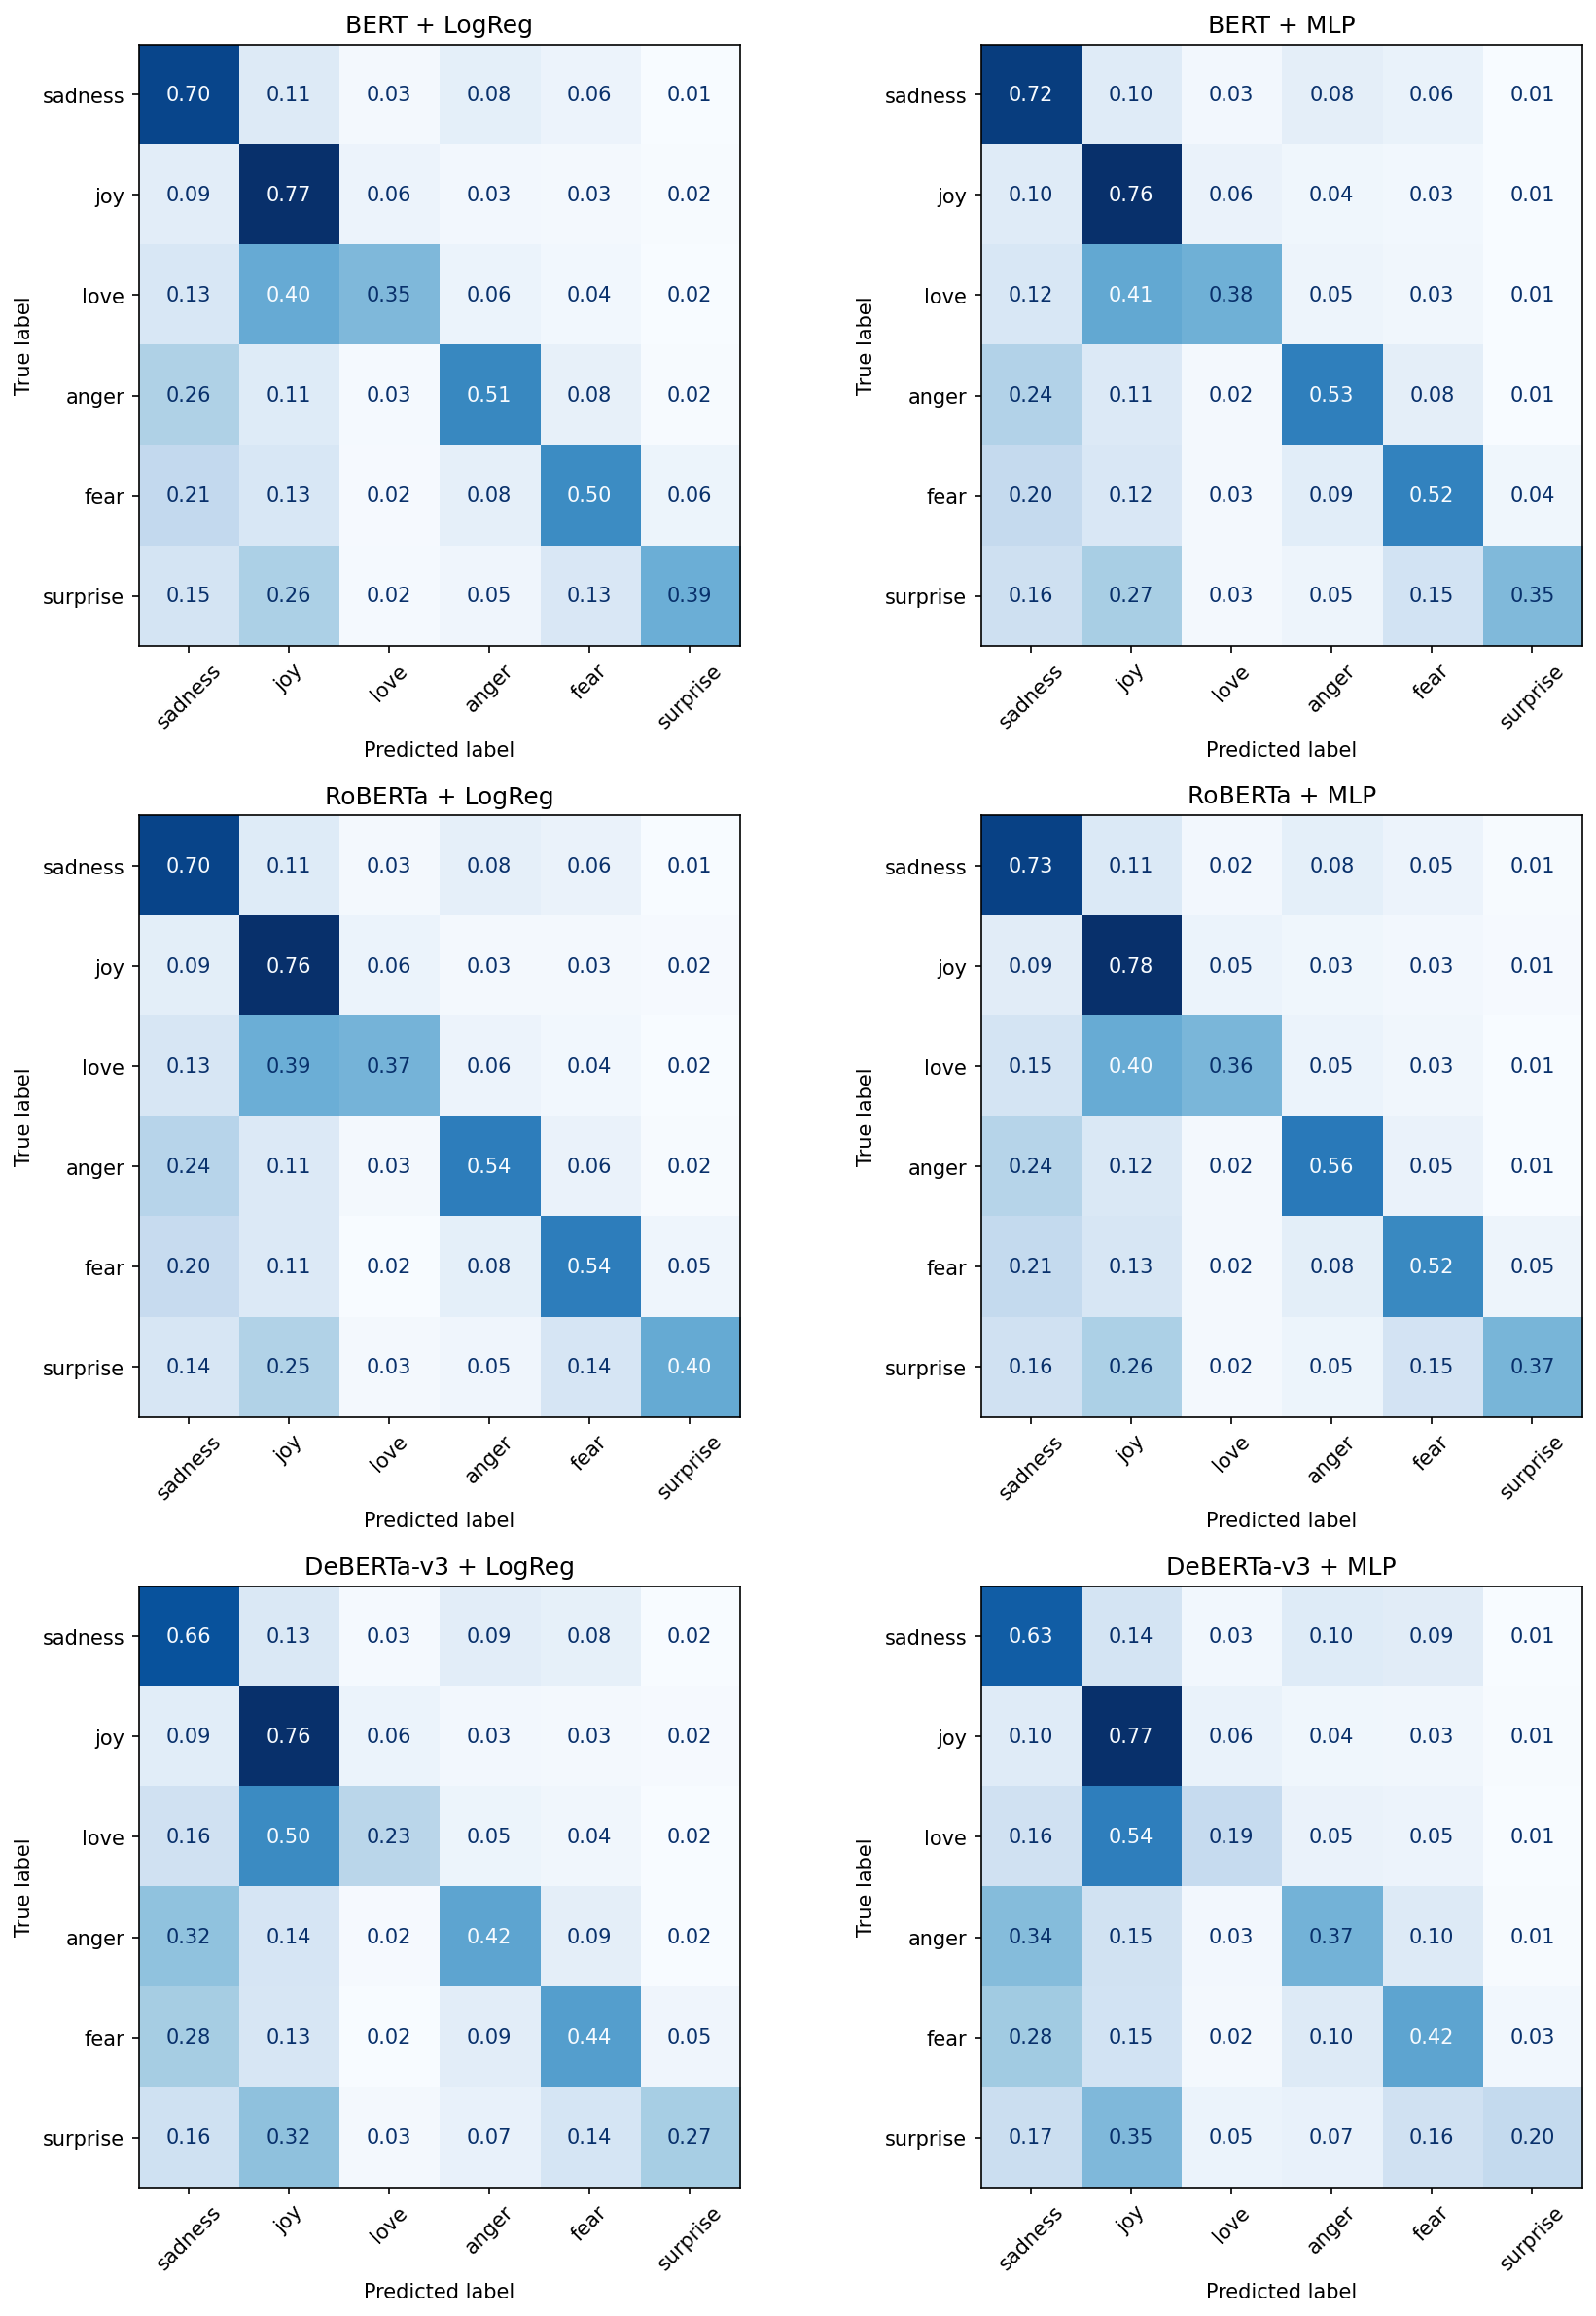
\includegraphics[width=0.74\textwidth]{confusion_normalized.png}
\caption{Matrizes de confusão das seis configurações com predições de validação dos 5 folds, normalizadas pela classe verdadeira (linhas).}
\label{fig:cm}
\end{figure}

\section{Discussão}

\paragraph{Encoders.} RoBERTa foi o melhor encoder com os dois classificadores, seguido de perto pelo BERT. A vantagem do RoBERTa (cerca de 0,01 de F1) é consistente com seu pré-treino em mais dados e mais diversos, incluindo texto da web mais próximo da linguagem informal de tweets. Ainda assim, ela tem a mesma ordem do desvio-padrão entre folds, então RoBERTa + MLP, RoBERTa + LogReg e BERT + MLP devem ser vistos como praticamente empatados.

O resultado mais marcante é o DeBERTa-v3, cerca de 0,09 a 0,13 de F1 abaixo dos outros, embora seja o mais forte dos três quando ajustado (fine-tuning) em benchmarks como o GLUE. Atribuímos isso ao objetivo de pré-treino. Na detecção de token substituído, a última camada é especializada em decidir, token a token, se aquele token é original ou trocado, e não em codificar o significado da frase de forma que sobreviva a uma média. Seus estados ocultos são ótimos pontos de partida para ajuste fino, mas pouco informativos quando congelados e combinados por mean pooling. Verificamos que a tokenização estava correta, então a diferença não é artefato de implementação. Isso mostra que o desempenho após ajuste fino não prevê a qualidade da representação congelada.

\paragraph{Classificadores.} Com BERT e RoBERTa, o MLP superou a regressão logística por cerca de 0,01 de F1 e 0,01 de acurácia, um ganho pequeno: a maior parte da informação útil já é linearmente acessível e a camada não linear acrescenta pouco. O MLP também teve variância maior entre folds, efeito do \textit{early stopping} com uma validação interna pequena. Com DeBERTa-v3 a ordem se inverte e a regressão logística é melhor: quando o sinal é fraco, a capacidade extra do MLP ajusta ruído, e o modelo linear regularizado generaliza melhor. O MLP também tende a favorecer as classes majoritárias (precisão maior que recall), o que piora \textit{love} e \textit{surprise} no DeBERTa-v3.

\paragraph{Classes e erros.} Em todas as configurações, \textit{joy} e \textit{sadness} têm o melhor F1 (0,70 a 0,75) e \textit{love} e \textit{surprise} o pior (0,24 a 0,42). As matrizes de confusão mostram padrões coerentes entre os encoders: cerca de 40\% de \textit{love} vai para \textit{joy} (são emoções positivas próximas e \textit{love} tem um quinto dos exemplos), \textit{surprise} se espalha entre \textit{joy} e \textit{fear}, e cerca de um quarto de \textit{anger} e \textit{fear} é classificado como \textit{sadness}, a classe negativa mais frequente. Isso explica por que o F1 macro (0,56) fica bem abaixo da acurácia (0,65): os erros se concentram nas classes minoritárias, que pesam igual na média macro. O ruído dos rótulos por hashtag e a remoção da pontuação, que carrega informação emocional, também limitam o teto alcançável.

\paragraph{Limitações.} Usamos apenas a última camada e mean pooling. Camadas intermediárias ou a concatenação de várias camadas costumam dar representações congeladas melhores, sobretudo para o DeBERTa-v3. Não ajustamos hiperparâmetros nem compensamos o desbalanceamento (por exemplo com \texttt{class\_weight="balanced"} na regressão logística), o que provavelmente elevaria o recall das classes minoritárias. Como referência, encoders do mesmo porte ajustados de ponta a ponta chegam a acurácia acima de 0,90 neste dataset, então o congelamento custa muito nesta tarefa.

\section{Conclusões}

Entre as seis configurações, RoBERTa + MLP obteve o melhor desempenho (acurácia 0,654 e F1 macro 0,569), mas praticamente empatado com RoBERTa + LogReg e BERT + MLP. A escolha do encoder pesou muito mais que a do classificador: trocar regressão logística por MLP mudou o F1 em cerca de 0,01, enquanto trocar BERT ou RoBERTa por DeBERTa-v3 custou mais de 0,08. O principal aprendizado é que a qualidade de um encoder congelado depende do seu objetivo de pré-treino, e que modelos pré-treinados como discriminadores (estilo ELECTRA) são uma má escolha para extração de características sem ajuste fino. As classes minoritárias e semanticamente próximas (\textit{love}, \textit{surprise}) concentram os erros em todos os casos.

\section*{Referências}
\small
\begin{itemize}[leftmargin=*]
\item Saravia, E., Liu, H.-C. T., Huang, Y.-H., Wu, J., Chen, Y.-S. CARER: Contextualized Affect Representations for Emotion Recognition. EMNLP, 2018.
\item Devlin, J., Chang, M.-W., Lee, K., Toutanova, K. BERT: Pre-training of Deep Bidirectional Transformers for Language Understanding. NAACL, 2019.
\item Liu, Y. et al. RoBERTa: A Robustly Optimized BERT Pretraining Approach. arXiv:1907.11692, 2019.
\item He, P., Gao, J., Chen, W. DeBERTaV3: Improving DeBERTa using ELECTRA-Style Pre-Training with Gradient-Disentangled Embedding Sharing. ICLR, 2023.
\item Pedregosa, F. et al. Scikit-learn: Machine Learning in Python. JMLR, 2011. Wolf, T. et al. Transformers: State-of-the-Art Natural Language Processing. EMNLP (Demos), 2020.
\end{itemize}

\end{document}
